\section{切割与黏合}
\label{ch12-sec76}

为了证明分类定理, 我们需要用到某种几何方法, 这便是所谓"切割"与"黏合"的方法. 这些技巧将说明如何将一个或多个多边形区域根据给定的标记表黏合多边形的边来获得一个空间 $X$, 以及如何用多边形区域和标记表来表示 $X$.

首先我们说明把一个多边形区域"切割"是什么意思. 设 $P$ 是一个多边形区域, 其顶点依次为 $p_{0},\ \cdots,\ p_{n}=p_{0}$. 给定 $k$, $1<k<n-1$, 考虑依次以 $p_{0},\ \cdots,\ p_{k},\ p_{0}$ 为顶点的多边形区域 $Q_{1}$ 和依次以 $p_{0},\ p_{k},\ \cdots,\ p_{n}=p_{0}$ 为顶点的多边形区域 $Q_{2}$. 这两个区域有公共边 $p_{0}p_{k}$, 并且区域 $P$ 是它们的并.

用 $\mathbb{R}^{2}$ 的一个变换将 $Q_{1}$ 移动, 要求 $Q_{1}$ 移动到的多边形区域 $Q_{1}'$ 与 $Q_{2}$ 无交. 这时区域 $Q_{1}'$ 依次以 $q_{0},\ q_{1},\ \cdots,\ q_{k},\ q_{0}$ 为顶点, 其中 $q_{i}$ 为 $p_{i}$ 在 $\mathbb{R}^{2}$ 的变换下的像. 将区域 $Q_{1}'$ 和 $Q_{2}$ 称为 $P$ 沿从 $p_{0}$ 到 $p_{k}$ 的直线\textbf{切割}(cut)而得到的两个区域. 这时, 区域 $P$ 同胚于 $Q_{1}'\cup Q_{2}$ 的一个商空间, 它是将 $Q_{1}'$ 中从 $q_{0}$ 到 $q_{k}$ 的那条边与 $Q_{2}$ 中从 $p_{0}$ 到 $p_{k}$ 的那条边按照这两条边之间正线性映射的方式黏合起来而得到的. 参见\cref{ch12-fig-76-1}.

\par
\begin{figure}[htbp]
\centering
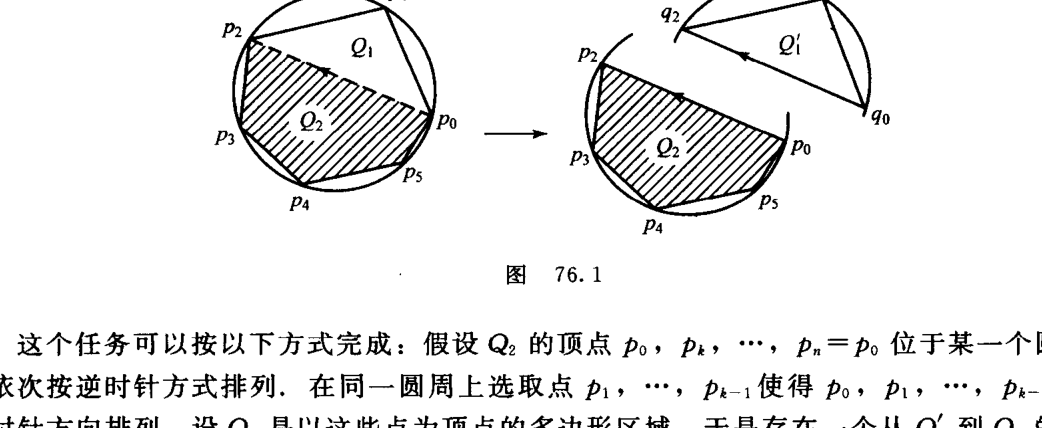
\includegraphics[width=0.7\textwidth]{image/fig-76-1.png}
\caption{沿 $p_{0}p_{k}$ 切割多边形区域.}
\label{ch12-fig-76-1}
\end{figure}

现在我们来考虑上述过程的逆过程. 假设给定两个无交的多边形区域 $Q_{1}'$ 和 $Q_{2}$, 它们的顶点依次为 $q_{0},\ \cdots,\ q_{k},\ q_{0}$ 和 $p_{0},\ p_{k},\ \cdots,\ p_{n}=p_{0}$. 并且假定有一个商空间是将 $Q_{1}'$ 中从 $q_{0}$ 到 $q_{k}$ 的那条边与 $Q_{2}$ 中从 $p_{0}$ 到 $p_{k}$ 的那条边按照这两条边之间正线性映射的方式黏合起来而得到的. 我们希望用一个多边形区域 $P$ 表示这个空间.

这个任务可以按以下方式完成: 假设 $Q_{2}$ 的顶点 $p_{0},\ p_{k},\ \cdots,\ p_{n}=p_{0}$ 位于某一个圆周上并且依次按逆时针方式排列. 在同一圆周上选取点 $p_{1},\ \cdots,\ p_{k-1}$ 使得 $p_{0},\ p_{1},\ \cdots,\ p_{k-1},\ p_{k}$ 依逆时针方向排列. 设 $Q_{1}$ 是以这些点为顶点的多边形区域. 于是存在一个从 $Q_{1}'$ 到 $Q_{1}$ 的同胚将每一个 $q_{i}$ 映为 $p_{i}$, 并且将 $Q_{1}'$ 的边 $q_{0}q_{k}$ 线性地映为 $Q_{2}$ 的边 $p_{0}p_{k}$. 此时上一段中提到的商空间便同胚于区域 $P$, 它是 $Q_{1}$ 与 $Q_{2}$ 的并. 我们称 $P$ 为沿着指定的两条边将 $Q_{1}'$ 和 $Q_{2}$ \textbf{黏合}(paste)起来而得到的. 参见\cref{ch12-fig-76-2}.

\par
\begin{figure}[htbp]
\centering
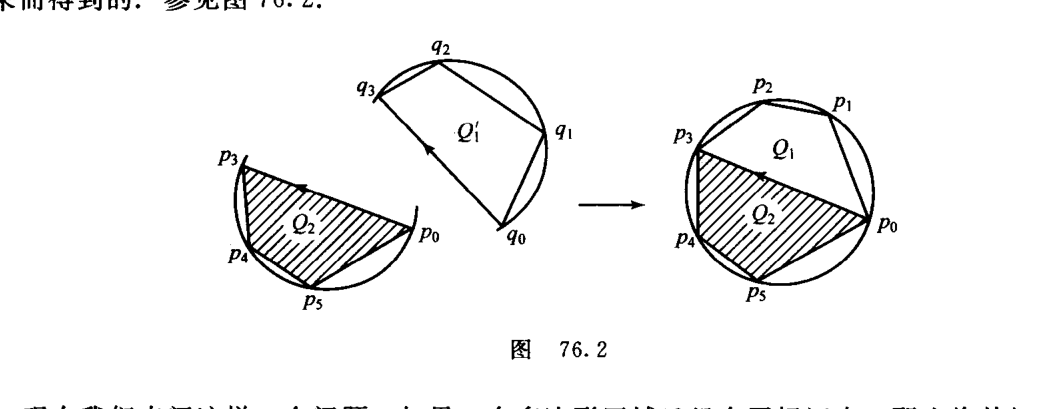
\includegraphics[width=0.75\textwidth]{image/fig-76-2.png}
\caption{将两个区域沿指定的边黏合.}
\label{ch12-fig-76-2}
\end{figure}

现在我们来问这样一个问题: 如果一个多边形区域已经有了标记表, 那么将其切割后对标记表有怎样的影响? 更确切地说, 给定无交的多边形区域的一个族 $P_{1},\ \cdots,\ P_{m}$ 和这些区域的标记表 $w_{1},\ \cdots,\ w_{m}$, 其中 $w_{i}$ 为 $P_{i}$ 中诸边的标记表. 假设 $X$ 是借助于这些标记表所给出的商空间. 如果沿 $p_{0}p_{k}$ 将 $P_{1}$ 割开, 其影响是怎样的? 这时, 我们得到了 $m+1$ 个多边形区域 $Q_{1}'$, $Q_{2}$, $P_{2},\ \cdots,\ P_{m}$. 为了通过这些区域获得空间 $X$, 我们需要增加一对边的黏合. 为了表示出增加的这一对边的黏合, 我们需要增加一个标签, 并且将它分配给新引入的一对边 $q_{0}q_{k}$ 和 $p_{0}p_{k}$. 因为对 $Q_{2}$ 而言, 从 $p_{0}$ 到 $p_{k}$ 是逆时针方向. 对于 $Q_{1}'$ 而言, 从 $q_{0}$ 到 $q_{k}$ 为顺时针方向, 因此在 $Q_{2}$ 的标记表中相应的标签取指数 $+1$, 在 $Q_{1}'$ 的标记表中相应的标签取指数 $-1$.

让我们说得更明白些. 将 $P_{1}$ 的标记表 $w_{1}$ 写成 $w_{1}=y_{0}y_{1}$ 的形式, 其中 $y_{0}$ 为 $w_{1}$ 的前 $k$ 项, $y_{1}$ 为余下的部分. 设 $c$ 是一个在标记表 $w_{1},\ \cdots,\ w_{m}$ 的各项中都未曾使用的标记. 这时, 取 $Q_{1}'$ 的标记表为 $y_{0}c^{-1}$, 取 $Q_{2}$ 的标记表为 $cy_{1}$. 对于 $i>1$ 仍取区域 $P_{i}$ 上原有的标记表 $w_{i}$.

易见, 空间 $X$ 可以通过区域 $Q_{1}'$, $Q_{2}$, $P_{2},\ \cdots,\ P_{m}$ 借助于这个标记表来获得. 因为商映射的复合是一个商映射, 所以无论我们一次黏合所有的边, 还是先将 $p_{0}p_{k}$ 与 $q_{0}q_{k}$ 黏合然后再黏合其他边, 其结果都是一样的.

当然也可以将上述过程反过来运用. 如果 $X$ 是通过区域 $Q_{1}'$, $Q_{2}$, $P_{2},\ \cdots,\ P_{m}$ 借助于一个标记表来构成的, 这个标记表表明第一个区域的一条边与第二个区域的另一条边黏合(并且没有其他边被黏合到其上), 那么我们便可以先实施这个黏合. 这样一来 $X$ 便变成了 $m$ 个区域 $P_{1},\ \cdots,\ P_{m}$ 通过一个标记表得到的空间了.

将上述内容总结为以下定理.

\begin{theorem}[切割与黏合的等价性]
\label{theorem:ch12-cut-paste}
设 $X$ 是由 $m$ 个多边形区域借助于标记表
\[
y_{0}y_{1},w_{2},\cdots,w_m \qquad (*)
\]
通过边的黏合所得到的空间. 设标签 $c$ 不在这个标记表中出现. 若 $y_{0}$ 和 $y_{1}$ 的长度都不小于 $2$, 则 $X$ 也可以由 $m+1$ 个多边形区域借助于标记表
\[
y_{0}c^{-1},cy_{1},w_{2},\cdots,w_m \qquad (**)
\]
通过边的黏合而得到. 反之, 若 $X$ 是由 $m+1$ 个多边形区域借助于标记表 $(**)$ 通过边的黏合而得到的空间, 并且 $c$ 不在标记表 $(*)$ 中, 则 $X$ 也可以由 $m$ 个多边形区域借助于标记表 $(*)$ 得到.
\end{theorem}

\subsection*{标记表的初等运算}

下面列举一些初等运算, 它们作用于标记表 $w_{1},\ \cdots,\ w_{m}$ 时对于相应的商空间 $X$ 没有影响. 前两种运算是由 \cref{theorem:ch12-cut-paste} 给出的.

\begin{enumerate}[(i)]
\item \textbf{切割}. 将标记表 $w_{1}=y_{0}y_{1}$ 换成标记表 $y_{0}c^{-1}$ 和 $cy_{1}$, 其中 $c$ 在全部标记表中不出现, 并且 $y_{0}$ 和 $y_{1}$ 的长度均不小于 $2$.
\item \textbf{黏合}. 将标记表 $y_{0}c^{-1}$ 和 $cy_{1}$ 换成 $y_{0}y_{1}$, 其中 $c$ 在全部标记表的其他位置不出现.
\item \textbf{换标签}. 用某一个在全部标记表中未出现过的新的标签代替原标记表中出现的所有同一个标签. 类似地, 可以将一个给定的标签 $a$ 的所有指数同时改变符号. 这意味着重置标记为 $a$ 的所有边的方向. 这样做对黏合映射没有影响.
\item \textbf{置换}. 将一个标记表 $w_{i}$ 换成它的一个循环置换. 特别地, 若 $w_{i}=y_{0}y_{1}$, 我们可以用 $y_{1}y_{0}$ 代替 $w_{i}$. 这意味着从某一个顶点开始将多边形区域 $P_{i}$ 的诸顶点重新编号, 它对商空间没有影响.
\item \textbf{翻转}. 将标记表
\[
w_{i}=(a_{i_{1}})^{\varepsilon_{1}}\cdots(a_{i_{n}})^{\varepsilon_{n}}
\]
替换为它的形式逆
\[
w_{i}^{-1}=(a_{i_{n}})^{-\varepsilon_{n}}\cdots(a_{i_{1}})^{-\varepsilon_{1}}.
\]
这意味着"多边形区域 $P_{i}$ 翻了个个儿". 这时, 所有顶点的顺序翻转过来了, 并且对于所有边的定向也翻转过来了. 这不影响商空间 $X$.
\item \textbf{删除}. 将标记表 $w_{i}=y_{0}aa^{-1}y_{1}$ 替换为 $y_{0}y_{1}$, 其中 $a$ 在全部标记表的其他位置不出现, 并且 $y_{0}$ 和 $y_{1}$ 的长度均不小于 $2$.
\end{enumerate}

最后这个结论可以根据\cref{ch12-fig-76-3} 中所示的三个步骤予以说明, 只有一个步骤以前没有提到过. 设 $b$ 和 $c$ 是在全部标记表中不出现的两个标签. 先通过切割运算 (i) 用 $y_{0}ab$ 替换 $y_{0}aa^{-1}y_{1}$ 和 $b^{-1}a^{-1}y_{1}$, 然后在每一个多边形区域中将以 $a$ 和 $b$ 为标签的两条边分别合并成一条边, 并且赋予一个新的标签. 这一步是新的. 其结果是得到两个标记表 $y_{0}c$ 和 $c^{-1}y_{1}$, 它们可以通过黏合运算 (ii) 被换成一个标记表 $y_{0}y_{1}$.

\par
\begin{figure}[htbp]
\centering
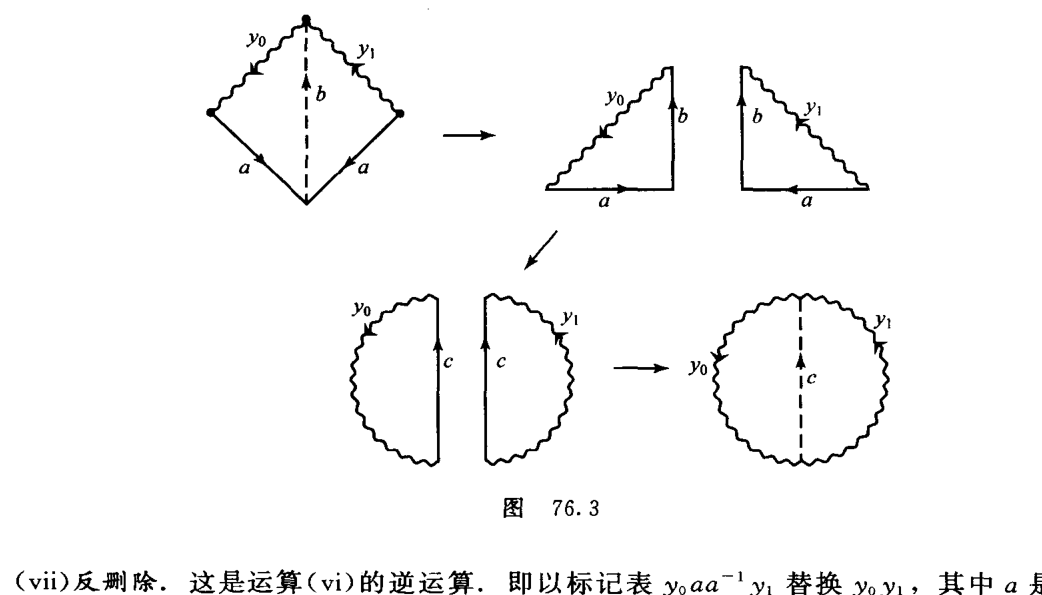
\includegraphics[width=0.7\textwidth]{image/fig-76-3.png}
\caption{删除运算的三个步骤.}
\label{ch12-fig-76-3}
\end{figure}

\begin{enumerate}[(i)]
\setcounter{enumi}{6}
\item \textbf{反删除}. 这是运算 (vi) 的逆运算. 即以标记表 $y_{0}aa^{-1}y_{1}$ 替换 $y_{0}y_{1}$, 其中 $a$ 是在全部标记表中没有出现过的一个标签. 实际上我们不会用到这个运算.
\end{enumerate}

\begin{definition}[等价的标记表]
\label{definition:ch12-equivalent-schemes}
我们称标记两族多边形区域的两个标记表是\textbf{等价的}(equivalent), 如果可以经过一系列的初等运算将其中一个标记表化为另一个. 由于每一个初等运算的逆运算也是一个初等运算, 所以上述关系是一个等价关系.
\end{definition}

\begin{example}[Klein 瓶的化简]
\label{example:ch12-klein-reduction}
Klein 瓶 $K$ 是通过标记表 $aba^{-1}b$ 得到的空间. 在第 74 节中, 曾经求证 $K$ 同胚于 $2$-重射影平面 $P^{2}\#P^{2}$. 事实上, 这个问题的几何证明可归结为下列初等运算:
\begin{align*}
aba^{-1}b\quad&\longrightarrow\quad abc^{-1}\ \text{和}\ ca^{-1}b &&\text{切割}\\
&\longrightarrow\quad c^{-1}ab\ \text{和}\ b^{-1}ac^{-1} &&\text{置换和翻转}\\
&\longrightarrow\quad c^{-1}aac^{-1} &&\text{黏合}\\
&\longrightarrow\quad aacc &&\text{置换和换标签}.
\end{align*}
\end{example}

\begin{exercise}
\label{exercise:ch12-sec76-01}
考虑商空间 $X$, 它是两个多边形区域借助于标记表 $w_{1}=acbc^{-1}$ 和 $w_{2}=cdba^{-1}d$ 得到的.
\begin{enumerate}[(a)]
\item 如果将两个多边形区域中以"$a$"为标签的边黏合, 我们可将 $X$ 表示为一个 $7$-边形区域 $P$ 的商空间. $P$ 的标记表是怎样的? 通过哪些初等运算来得到新的标记表?
\item 将两个多边形区域中以"$b$"为标签的边黏合, 回答 (a) 中的相应问题.
\item 说明为什么不能通过黏合以"$c$"为标签的边来得到标记表 $acbdba^{-1}d$ 用以表示 $X$.
\end{enumerate}
\end{exercise}

\begin{exercise}
\label{exercise:ch12-sec76-02}
考虑两个多边形区域借助于标记表 $w_{1}=abcc$ 和 $w_{2}=c^{-1}c^{-1}ab$ 所得到的空间 $X$. 以下一系列初等运算
\begin{align*}
abcc\ \text{和}\ c^{-1}c^{-1}ab\quad&\longrightarrow\quad ccab\ \text{和}\ b^{-1}a^{-1}cc &&\text{置换和翻转}\\
&\longrightarrow\quad ccaa^{-1}cc &&\text{黏合}\\
&\longrightarrow\quad cccc &&\text{删除}
\end{align*}
说明 $X$ 同胚于 $4$-叠小丑帽. 一系列初等运算
\begin{align*}
abcc\ \text{和}\ c^{-1}c^{-1}ab\quad&\longrightarrow\quad abcc^{-1}ab &&\text{黏合}\\
&\longrightarrow\quad abab &&\text{删除}
\end{align*}
说明 $X$ 同胚于 $P^{2}$. 然而, 这两个空间不同胚. 以上两个推导中, 哪个是正确的?
\end{exercise}
